% Part 2 - Literature study

\chapter{Video Game Theory}
\label{chapter:lit-study-game-theory}
\lhead{Chapter \ref{chapter:lit-study-game-theory}. \emph{Video Game Theory}}

This chapter looks at some previous articles on subjects related to video game theory with the goal of establishing a terminology to be used throughout the project.

\section{Pervasive Games}

In today's multitude of game genres, \emph{pervasive games} is the one that is most relevant to this project. The definition of pervasive gaming is somewhat fluid. According to Benford et al. \cite{benford2005pervasive}, \emph{"Pervasive games extend the gaming experience out into the real world"}, further stating that \emph{"The game player becomes unchained from the console and experiences a game that is interwoven with the real world and is potentially available at any place and any time"}.

Montola \cite{montola2005exploring} describes a pervasive game as \emph{"a game that has one or more salient	features that expand the contractual magic circle of play socially, spatially or temporally"}. \emph{Spatial expansion} describes the concept of expanding the play area beyond the play device itself, using a larger location such as a city or, in some cases, the whole world. \emph{Temporal expansion} refers to the distribution of game play beyond traditional play sessions. Some games define every moment to be part of the game session, while others are inactive most of the time, being played only at certain times when the game itself decides. \emph{Social expansion} means the players can go beyond those who deliberately chose to participate in the game, turning bystanders into participants through various means.

Magerkurth et al. \cite{magerkurth2005pervasive} discuss the various sub-genres of pervasive gaming, including \emph{Smart Toys}, \emph{Affective Gaming} and \emph{Augmented Tabletop Games}. The main focus of this project, however, are the \emph{Location-Aware Games} and \emph{Augmented Reality Games}.

Location-aware games determine the player's position based on technology such as GPS, WiFi, or GSM signals, or short-range proximity-sensors using RFID, Bluetooth or similar. The player can then be placed on a large-scale game board, ranging from a city block or smaller, to the entire world, and can interact with the game by physically moving.

According to Bederson \cite{bederson1995ar}, \emph{"Augmented reality uses computers to enhance the richness of the real world. It differs from virtual reality in that it doesn’t attempt to replace the real world"}. Yuen et al. \cite{yuen2011augmented} said \emph{"Augmented reality (AR) refers to a wide spectrum of technologies that project computer generated materials, such as text, images, and video, onto users’ perceptions of the real world"}. Examples of augmented reality are superimposing 3D images on a camera view or playing audio based on the user's location and movement.

Kiefer et al. \cite{kiefer2006systematically} explored the design space of location-aware or location-based games, identifying three \emph{game design dimensions}, positing that new games can be created by choosing values for each of the three dimensions, or by taking an existing game and changing one of the dimensions. The first of the three dimensions is the dimension of \emph{game environmental embedding}, which \emph{"deals with the way the game world is embedded in the player’s environment"}, distinguishing between \emph{pure location-based games}, \emph{mixed reality location-based games} and \emph{augmented reality location-based games}.

They define a location-based game as \emph{"a game which is supported by localization technology and integrates the position of (one or several) players as main game element into its rules"}, focusing on the requirement that the game rules rely on the localization technology. Mixed reality location-based games refer to games where virtual objects affect the physical game space, but exist only in the virtual layer and cannot be perceived by the players in their physical location. Augmented reality location-based games on the other hand allow players to players to perceive the virtual game elements \emph{"from a first-person perspective"}.

The second dimension is the \emph{game conceptual dimension}, which refers to the concept and goals of the game, on a more specific level than the established game genres. They define four types game concepts for location-based games: \emph{Chase game}, \emph{Item hunt game}, \emph{Puzzle game} and \emph{Strategy game}. A chase game is a game were a player's physical speed is central in the pursuit of victory, and are typically technology-supported variants of the classic playground game of \emph{Tag}. Item hunt games involves the search for items hidden throughout the game board, while puzzle games have you solve one or more puzzles toward some ultimate goal. Strategy games require the player to plan their moves to win.

The third and final dimension is the \emph{spatial and temporal dimension}, where games can be either spatially continuous or discrete, and either temporally continuous or discrete. Spatially discrete (sd) games have game events take place only in specific locations, while spatially continuous (sc) games can progress the game anywhere. Similarly, temporally discrete (td) games allow movement in the game only at given moments, while temporally continuous (tc) games allow game progress and events at any time. They identified games with the \emph{sdtd}, \emph{sdtc} and \emph{sctc} combinations, but no \emph{sctd} games.

\section{Player Types}
\label{sec:player-types}

Player types are a way of categorizing players on various axes with the goal of creating an enjoyable game experience for the target audience. Identifying player types can also be important for developers of games whose business model is to sell in-game items rather than retail sale of the game itself, as Hamari \& Tuunanen \cite{hamari2014playertypes} discussed in their 2014 meta-synthesis on the subject. The design of such items is largely based on the potential customers, and what type of items will be sold will depend on who are going to play the game and what their motivations are.

There are countless studies on different player types, and Hamari \& Tuunanen \cite{hamari2014playertypes} compared the different ways previous researchers have segmented players to create their typologies, using primarily behavioral and psychographic segmentation, but sometimes also geographic or demographic segmentation.

They found that a common division was that of \emph{hardcore} and \emph{casual} players, but found this to be a too simplistic solution. Hardcore players were sometimes described to be more dedicated in all areas of the games, playing for longer sessions, more often and being more invested. However, they found that all these aspects and more were better treated separately, creating multiple scales used to define more than just two types of players.

Kallio et al. \cite{kallio2011gamermentalities} used a model consisting of the scales of \emph{Intensity} and \emph{Sociability}, along with a \emph{Games} component to define three different groups of gamer mentalities. The components of the model can be seen in Figure \ref{fig:kallio-gamer-mentalities-model}, as presented in their paper, and the three groups of mentalities they define using this model are \emph{Social mentality profiles}, \emph{Casual mentality profiles} and \emph{Commited mentality profiles}.

\begin{figure}[h]
	\centering
	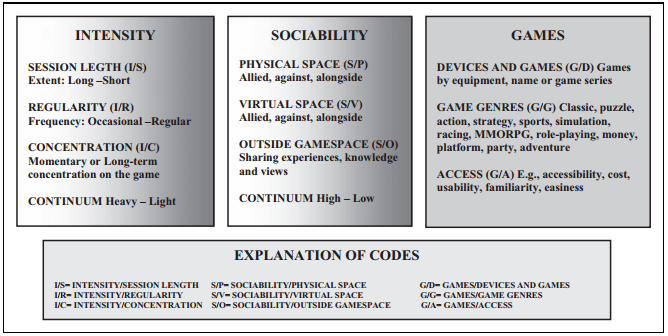
\includegraphics[width=\textwidth]{Figures/kallio-gaming-mentalities-model}
	\caption{The three components of gaming mentalities, as seen in Kallio et al. \cite{kallio2011gamermentalities}}
	\label{fig:kallio-gamer-mentalities-model}
\end{figure}

The social mentality profiles identified by Kallio et al. are of \emph{"quite light"} intensity, very high sociability and their choice in games focus on access to the games. The casual mentality profiles have variable intensity, low sociability and their choice in games focuses primarily on the device and access. The committed mentality profiles have \emph{"heavy"} intensity, high sociability and their choice in games focuses primarily on the genre. Each of the groups of profiles consist of three profiles with different, although similar, values for the various metrics defined in the model.

Hamari \& Tuunanen \cite{hamari2014playertypes} used this and other papers to identify a total of five \emph{"key dimensions pertaining to motivations of play/orientation of the player"}: \emph{Achievement}, \emph{Exploration}, \emph{Sociability}, \emph{Domination} and \emph{Immersion}.

In this project, we will use the five archetypal player types \emph{Achieving}, \emph{Exploring}, \emph{Socializing}, \emph{Dominating} and \emph{Immersing}, where each of them is \emph{more concerned with} their respective dimension of the game than the four others, rather than \emph{entirely focused on} only that aspect. That is, for a \emph{Socializing} player, the social aspect of the game is more important than any other aspect, but they may still have varying interest in the other four dimensions.

\section{Motivation in Gaming}
\label{sec:motivation-in-gaming}

When considering motivation, we typically distinguish between \emph{intrinsic} and \emph{extrinsic} motivation. \emph{Extrinsic motivation} is motivation from outside sources such as the promise of receiving rewards for successful completion of a task, or punishment should one fail to complete the task. \emph{Intrinsic motivation} on the other hand refers to motivation coming from within, where performing a task is in itself personally rewarding, either because it is fun, exciting, enjoyably challenging or a variety of other positive emotions.

Malone \cite{malone1981toward} proposes challenge, fantasy and curiosity as the primary factors of intrinsic motivation in gaming. Looking back at the player types established in Section \ref{sec:player-types}, the Achieving and Dominating players have challenge as their primary intrinsic motivator, while the Immersing player is motivated by fantasy and the Exploring player is motivated by curiosity. The Socializing player's main source of motivation is not related to the game itself.

While some studies suggest that extrinsic motivation can conflict with and undermine intrinsic motivation (see for example Benabou \& Tirole \cite{benabou2003intrinsic}, Lepper \& Henderlong \cite{lepper2000motivation}), extrinsic rewards are common in video games. By progressing or performing difficult tasks in games, players unlock new types of items or characters, receive powerful items or abilities, in-game currency, cosmetic modifications to their avatar, recognition from other players from being placed in a hall of fame or leader board of some kind, or any number of other rewards. For some, these rewards do indeed remove the fun - the intrinsic motivation - from the game, turning it into a chase for the next reward. For others, however, these rewards help bring back the fun they were no longer able to find, enjoying the game more when being rewarded.

In a market with hundreds of thousands of games and players with short attention spans, however, extrinsic rewards for small feats has become common. To keep players active, they are awarded for doing a minimal amount of effort every day through daily reward systems, often of the form \emph{First X of the day}. For some developers, this is the final step for the game: a last resort to keep players playing their game. For others, it is a means to bridge the gap until they can introduce new features.

% Chapter - Current state of physical and mental health in society (western world?)
\chapter{Health and Gaming}
\label{chapter:lit-study-modern-health}
\lhead{Chapter \ref{chapter:lit-study-modern-health}. \emph{Modern Society and Health}}

This chapter looks at some previous research on the effect of gaming on physical and mental health.

\section{Physical Activity}
\label{sec:lit-study-physical-activity}

Obesity is becoming an increasing problem as the world is further urbanized, and increasing physical inactivity is an important factor in the trend (Anderson \& Butcher \cite{anderson2006childhood}, Malik et al. \cite{malik2013global}, Uauy et al. \cite{uauy2001obesity}, Wang et al. \cite{wang2011health}). The World Health Organization (WHO) \cite{WHOobesity} report that worldwide obesity has more than doubled since 1980, with 39 \% of adults aged 18 years and older being overweight, and 13 \% being obese. To combat this, they recommend adults do \emph{"at least 150 minutes of moderate-intensity aerobic physical activity throughout the week"}, while children should do 60 minutes per day \cite{WHOphysical}. Janssen \& LeBlanc \cite{janssen2010systematic} performed a review of previous studies on \emph{"the relation between physical activity, fitness, and health in school-aged children and youth"}, and made similar recommendations based on these.

To motivate people to participate in physical activity, an emerging game trend in the last decade have been so-called \emph{exergames}. Whitehead et al. \cite{whitehead2010exergame} describe exergames as \emph{"video games that provide encouragement to exercise, particularly for an audience that may be reluctant to engage in the more traditional forms of exercise"}, further stating that \emph{"Exergames are a commonly accepted method of encouraging more physical activity to promote better health for those with high levels of sedentary screen time"}. Peng et al. \cite{peng2011playing} found that playing exergames were successful in increasing heart rate, oxygen consumption and energy expenditure to levels similar to those of traditional physical activities, and that they can \emph{"facilitate light- to moderate-intensity physical activity promotion"}.

\section{Mental Health}
\label{sec:lit-study-mental-health}

The WHO \cite{WHOdepression} estimate 350 million people worldwide suffering from depression, and the Anxiety and Depression Association of America (ADAA) \cite{ADAAanxiety} reports 18 \% of the US population suffering from anxiety disorders. These are serious disorders, and can in the worst case lead to suicide, yet less than half of those suffering, and in some countries fewer than 10 \% \cite{WHOdepression}, receive treatment for their condition.

Studies show that exercise can have a positive effect on depression, moderately to significantly reducing symptoms (Babyak et al. \cite{babyak2000exercise}, Dunn et al. \cite{dunn2005exercise}, Cooney et al. \cite{cooney2014exercise}), while Petruzzello et al. \cite{petruzzello1991meta}, Salmon \cite{salmon2001effects}, and Ströhle \cite{strohle2009physical} also found potential for a positive effect on anxiety disorders.

Rosenberg et al. \cite{rosenberg2010exergames} found potential for exergames to significantly improve symptoms of depression among elderly, and Brox et al. \cite{brox2011exergames} used exergames to a combined effect of increasing physical activity and decreasing loneliness among elderly.


% Chapter - Similar games
\chapter{Similar Games}
\label{chapter:lit-study-similar-games}
\lhead{Chapter \ref{chapter:lit-study-similar-games}. \emph{Game Types}}

This chapter looks at some games that are relevant to compare with Pokémon GO, for the most part miscellaneous pervasive games. Some games are more similar than others, but all of them share some aspect with Pokémon GO, be it the play style, game concepts or the device used to play.

\section{Ingress}
\label{sec:ingress}

Ingress is a location-aware, augmented reality game for Android and iOS phones. Like Pokémon GO, it was developed by Niantic Labs while it was a part of \emph{Google}. It was first officially released on Android in December 2013, and is considered by many to be the precursor to Pokémon GO. In an interview in October 2013 \cite{gamasutraBadger}, the product manager of Ingress stated that \emph{"Our vision for this, from Niantic Labs, is really to build a platform and to help other game studios, other developers, build similar types of geo-games on top of this infrastructure"}. Not only was it one of the first augmented reality games for mobile devices to enjoy commercial success, but it also laid the groundwork for more games to come.

The game narrative explains that so-called \emph{Exotic Matter (XM)} is spreading across the world from \emph{Portals}, and have been linked to an unseen alien race called \emph{the Shapers}. The players choose between two teams: the \emph{Enlightened}, who embrace the alien influence, and the \emph{Resistance}, who wish to save the human race from their \emph{ingress} into our world. The portals and exotic matter are visible through the player's \emph{scanner}, which is the mobile device the game is installed on.

\begin{figure}[h]
	\centering
	\begin{subfigure}[b]{0.3\textwidth}
		\centering
		
\includegraphics{Figures/ingress-logo}
		\caption{The Ingress logo}
	\end{subfigure}
	~
	\begin{subfigure}[t]{0.3\textwidth}
		\centering
		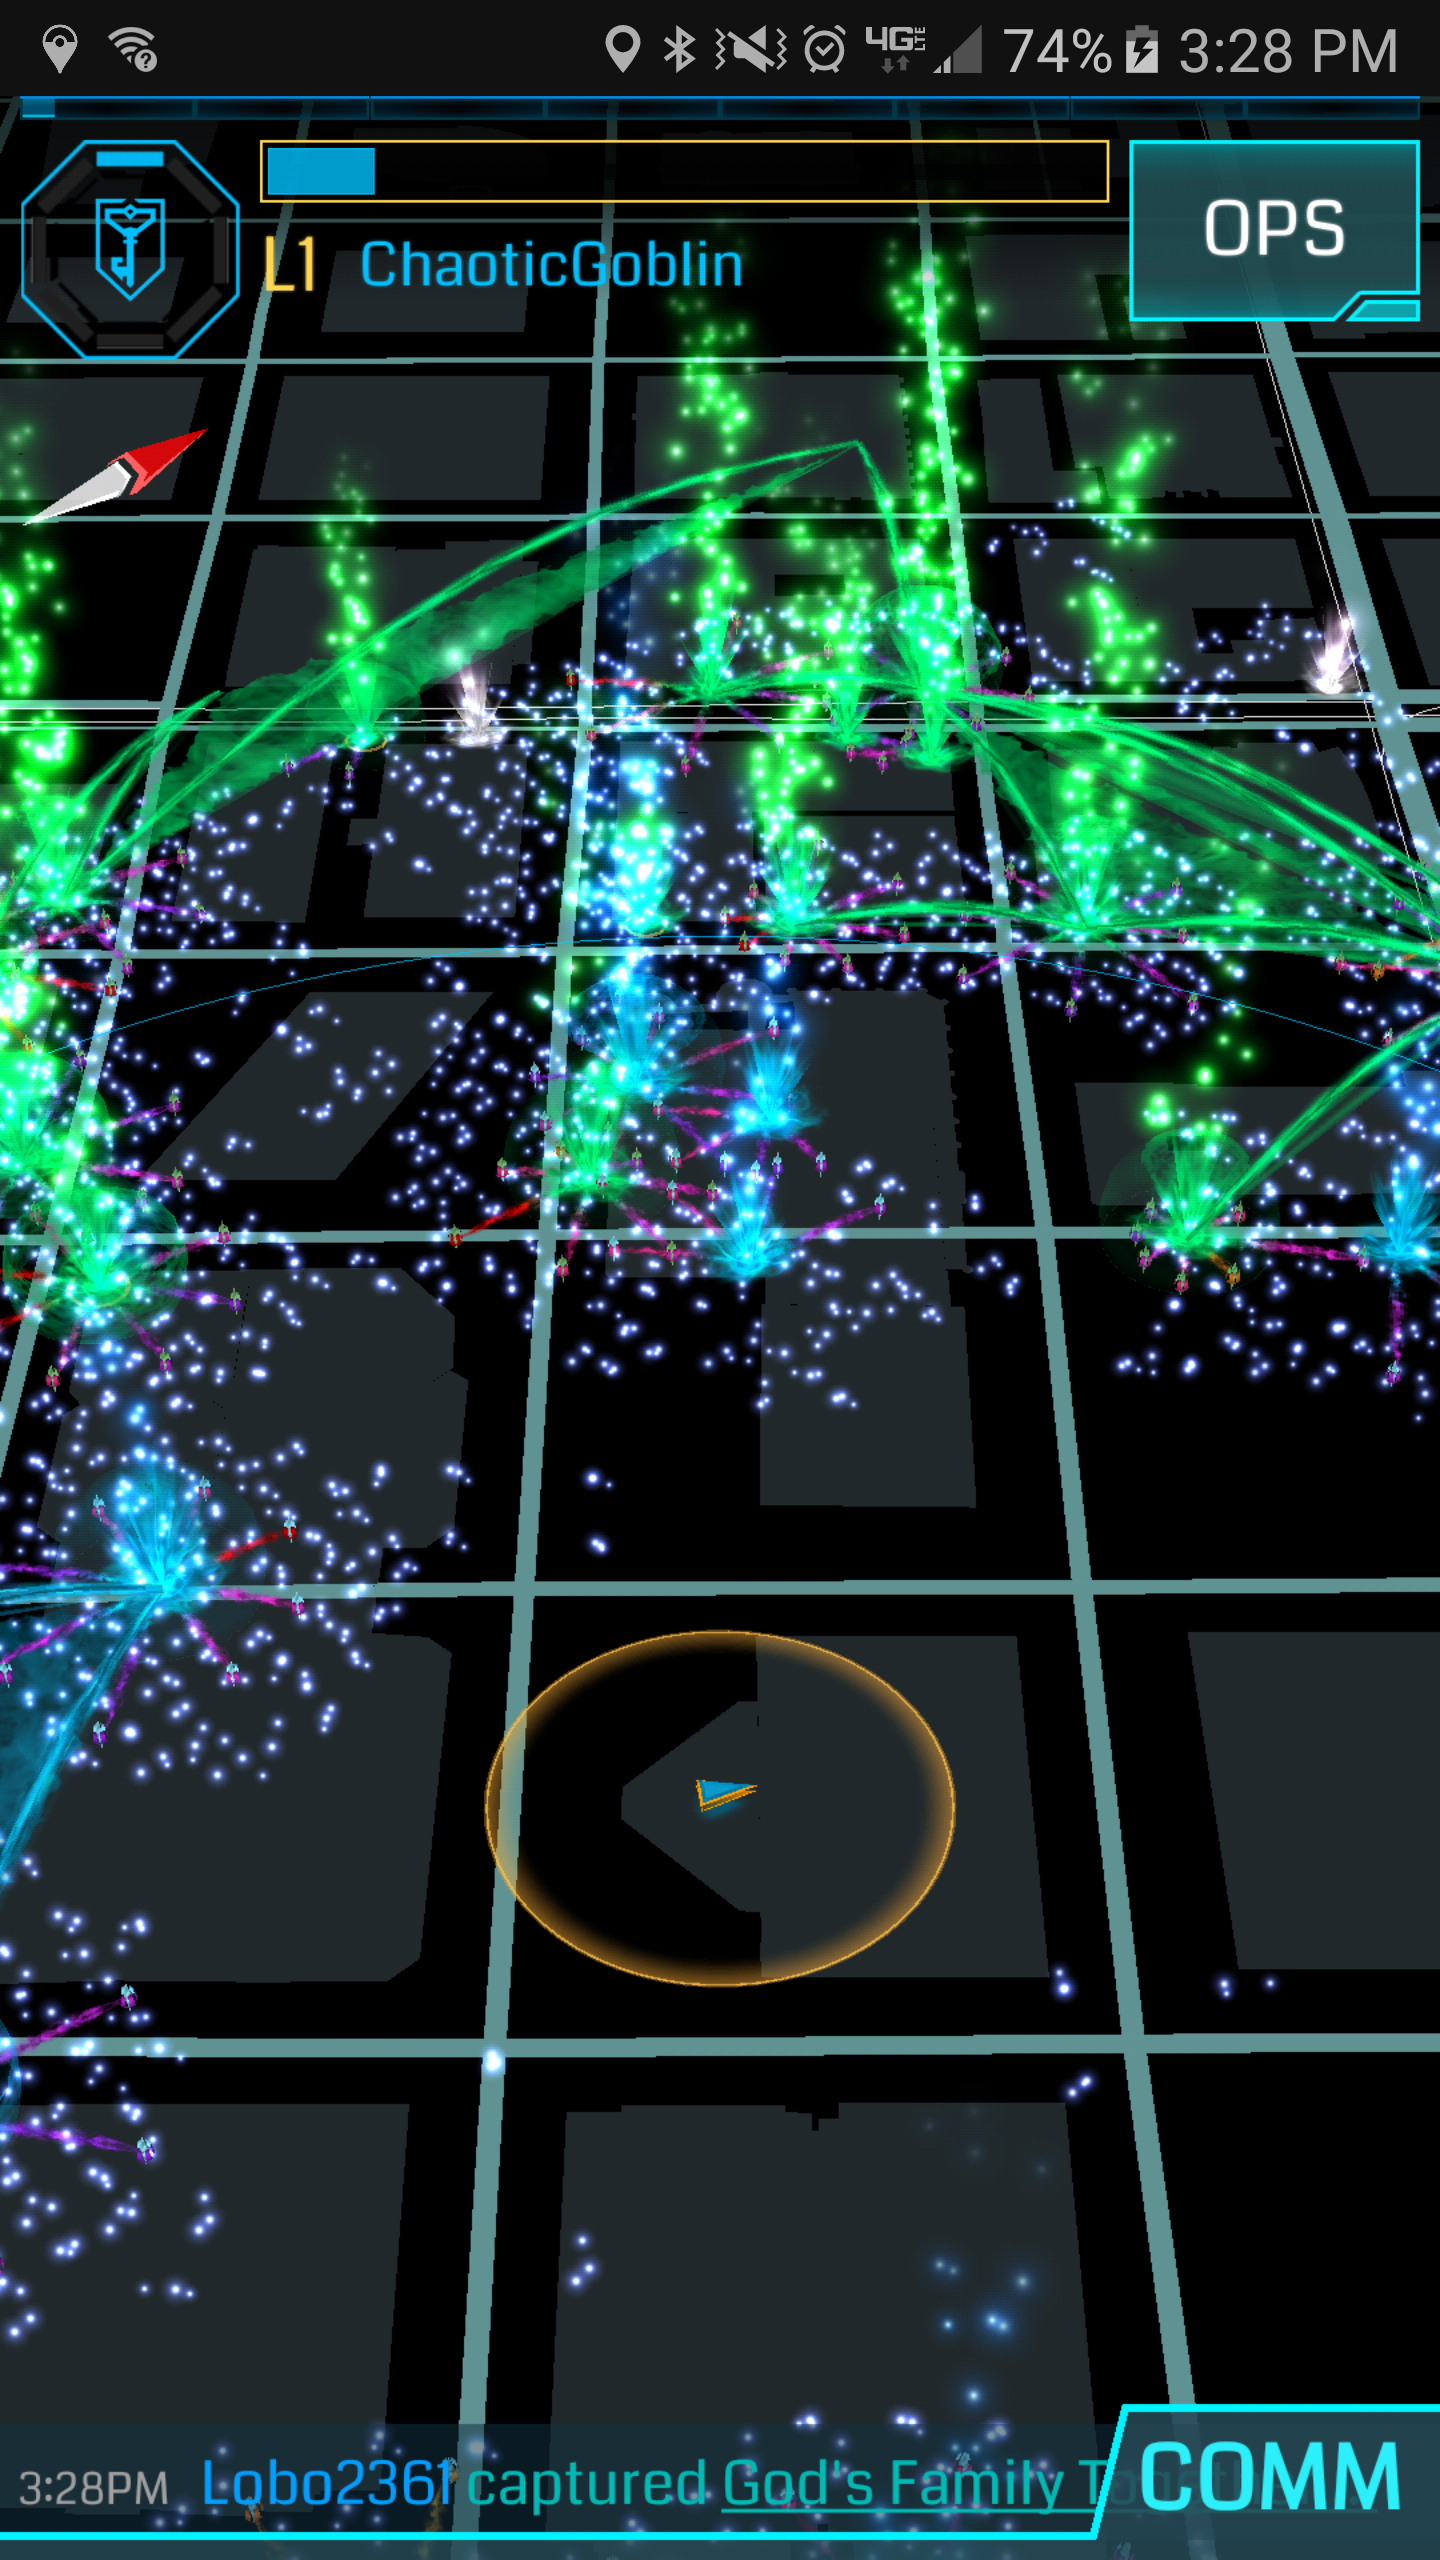
\includegraphics[height=3in]{Figures/chaoticgoblin-ingress-screenshot}
		\caption{A screenshot of an area with many portals and links, by Reddit user chaoticgoblin}
	\end{subfigure}
	~
	\begin{subfigure}[t]{0.3\textwidth}
		\centering
		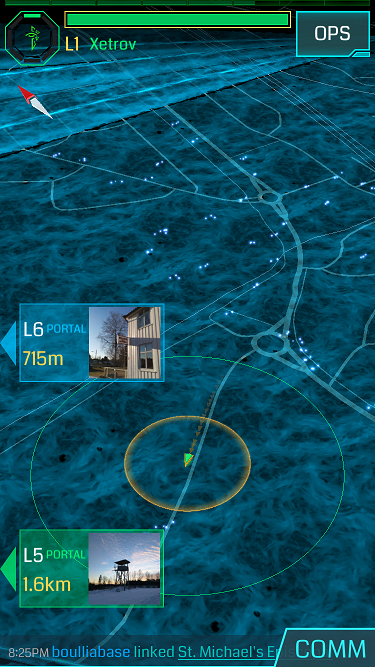
\includegraphics[height=3in]{Figures/ingress-fielded-area}
		\caption{A screenshot of an area covered by a field}
	\end{subfigure}
	\caption{Ingress}
\end{figure}

The game revolves around these portals, which players can \emph{hack} to retrieve items that help them claim these and other portals, while the XM they collect by moving around can be used to damage enemy portals. When a team is in complete control of multiple portals, players from that team can \emph{link} these portals to create a \emph{field}. Creating a field will claim the \emph{mind units} under the field for that team.

Portals in the game can be found at landmarks or points of interest, such as statues or buildings of note. Initially, the portals were based on \emph{"historical markers"}, but players could submit locations with descriptions to Niantic, and many of these were added to the game as portals \cite{mashableHanke}. Portal locations were also added later in conjunction with partnerships with various commercial chains such as \emph{Vodafone} \cite{auroraPromotion} or \emph{Jamba Juice}.

Progress in the game comes from performing actions, which yield \emph{action points (AP)} or earning \emph{badges} through achieving specific feats such as holding a friendly portal for a certain amount of time. The rewards for advancing in level is unlocking new, better items, and the only way to advance past level 9 (out of 16) is through earning badges.

Using Kiefer et al.'s \cite{kiefer2006systematically} game dimensions, the game is a \emph{strategy} more than anything else, requiring a solid plan if one wishes to have control over large areas. Although the game is referred to as an augmented reality game, using Kiefer et al.'s definitions, it is closer to a mixed reality game. XM is not perceptible in the real world, nor are the links or fields created. The portals are visible in the real world, but only in the capacity that they are real life objects, and this capacity does not depend on the game. Thus we have to argue that this is a \emph{mixed reality game}. If we ignore the XM, the game is spatially discrete, with game actions only taking place around portals. The collection of XM, however, is spatially continuous, as it can and will be collected mostly anywhere a player goes with the game open. The game is temporally continuous, with actions taking place at any time, although the game restricts the number of actions that can be taken on the same portal in a given time span. \emph{Anomalies}, special events inside and outside the game, take place at specific times, being temporally discrete.

The game is free to play, and earns revenue through an in-game store selling items for use in the game, an online store selling game-related merchandise, and partnerships with businesses that gain benefits such as portals at all their retail locations.

\section{Field Trip}

Another application developed by Niantic is Field Trip. It is not really a game in the way that most people think about games. It does not have rules, goals or other players. It is simply a tool that assists you in exploring. The app encourages you to explore by walking off in any arbitrary direction. When you get close to somewhere interesting, it notifies you. You can set preferences for what type of locations you are interested in, such as \emph{Architecture}, \emph{Historic Places \& Events} or \emph{Cool \& Unique}, and it will ignore other types of places while more frequently notifying you of these types of places.

\begin{figure}[h]
	\centering
	
\includegraphics[width=\textwidth]{Figures/fieldtrip-logo}
	\caption{The Field Trip logo}
\end{figure}

While the application is not a traditional game, it is worth mentioning not only because of its affiliation with Niantic, but because of its integration with Google's augmented reality device \emph{Google Glass}. With Field Trip, the Glasses show you \emph{cards} of the locations you encounter overlaid over what you usually would see, right in front of your eyes without requiring you to look at your phone or a similarly carried device.

Field Trip is also relevant in the way it encourages physical activity by suggesting you walk off in a random direction to explore, rather than find specific places before going out and traveling directly to them, something that often involves less physically exerting modes of transportation. Given that you are exploring somewhere with locations within your field of interest registered in Google's databases, Field Trip rewards you for your (potentially unintended) exercise with new, possibly exciting locations. These features resemble those of some exergames, motivating "players" to exercise through untraditional means.

\section{Geocaching}

Geocaching is a popular family activity game similar to the sport \emph{orienteering}. It is a game played with real life objects, but uses a mobile application to register the location of the items. The application lets you see a map of caches in an area, register your findings and make lists for a planned session. The caches are containers placed at any location, and are typically hidden somewhere clever in this location. The containers contain a logbook which the finder signs with their codename and time they found the cache, while some larger caches also contain trinkets or items that players can trade for one of their own items. Some caches require that you solve puzzles in the app before its exact coordinates are revealed to you.

\begin{figure}[h]
	\centering
	\begin{subfigure}[t]{0.5\textwidth}
		
\includegraphics[height=2.5in]{Figures/chaoticgoblin-geocache-covered}
		\caption{Cache covered in natural camouflage}
	\end{subfigure}
	~
	\begin{subfigure}[t]{0.4\textwidth}
		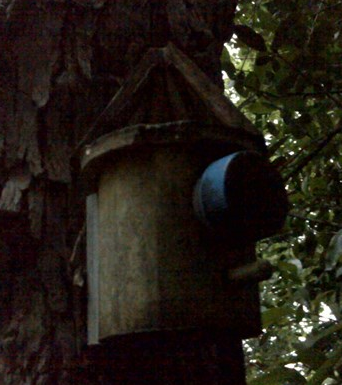
\includegraphics[height=2.5in]{Figures/chaoticgoblin-geocache-birdhouse}
		\caption{Cache hidden in birdhouse}
	\end{subfigure}
	~
	\begin{subfigure}[t]{\textwidth}
		\centering
		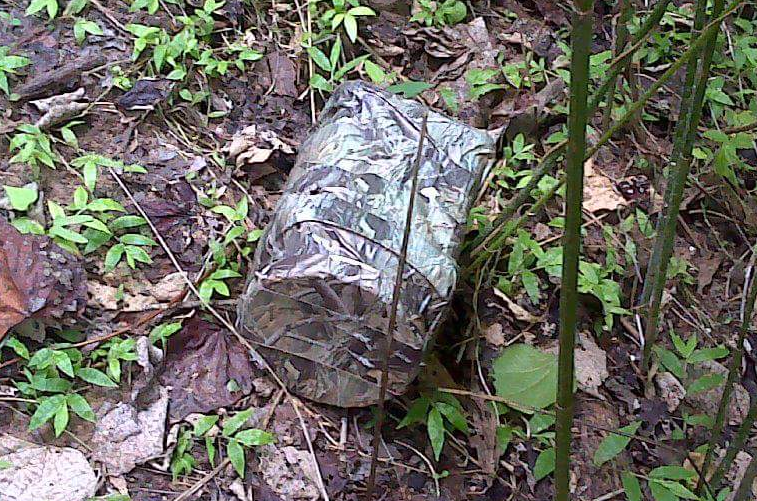
\includegraphics[height=2.5in]{Figures/chaoticgoblin-geocache-camo}
		\caption{Cache in camouflage-taped container}
	\end{subfigure}
	\caption{Clever hiding spots for geocaches (by Reddit user chaoticgoblin)}
	\label{fig:geocache-spots}
\end{figure}

Going back to Kiefer et al.'s \cite{kiefer2006systematically} dimensions for location-based games, Geocaching is primarily an item hunt game, and is in fact used as the most prominent example of one in their paper. Figure \ref{fig:geocache-spots} shows three clever hiding spots for caches found by Reddit user \emph{chaoticgoblin}, intended to make the player really have to search to find them. However, with the addition of caches that require you to solve puzzles to reveal their coordinates, Geocaching also gains aspects of a puzzle game. It is a pure location-based game, using localization technology solely to inform players of the location of the physical items, items that have no virtual equivalent. While caches technically can be placed anywhere, the actual locations of caches, where game events take place, are discrete and fairly static. Creating and placing a new cache can be done anywhere, but once placed, the location is discrete. Thus we classify Geocaching as spatially discrete. The game can be played at any time, and is thus temporally continuous.

Geocaching is free to play, and earns its revenue through partnerships with businesses and the sale of access to premium features such as making lists in the application to plan play sessions.

\section{Zombies, Run!}

Zombies, Run! is an exergame for Android and iOS devices. First released in 2012, it has added a new \emph{season} of content each year since, and now has 200 missions to play through. Within two weeks of its release, it was the highest grossing app in the Health \& Fitness category in the iOS App Store, and now has a million players.

\begin{figure}[h]
	\centering
	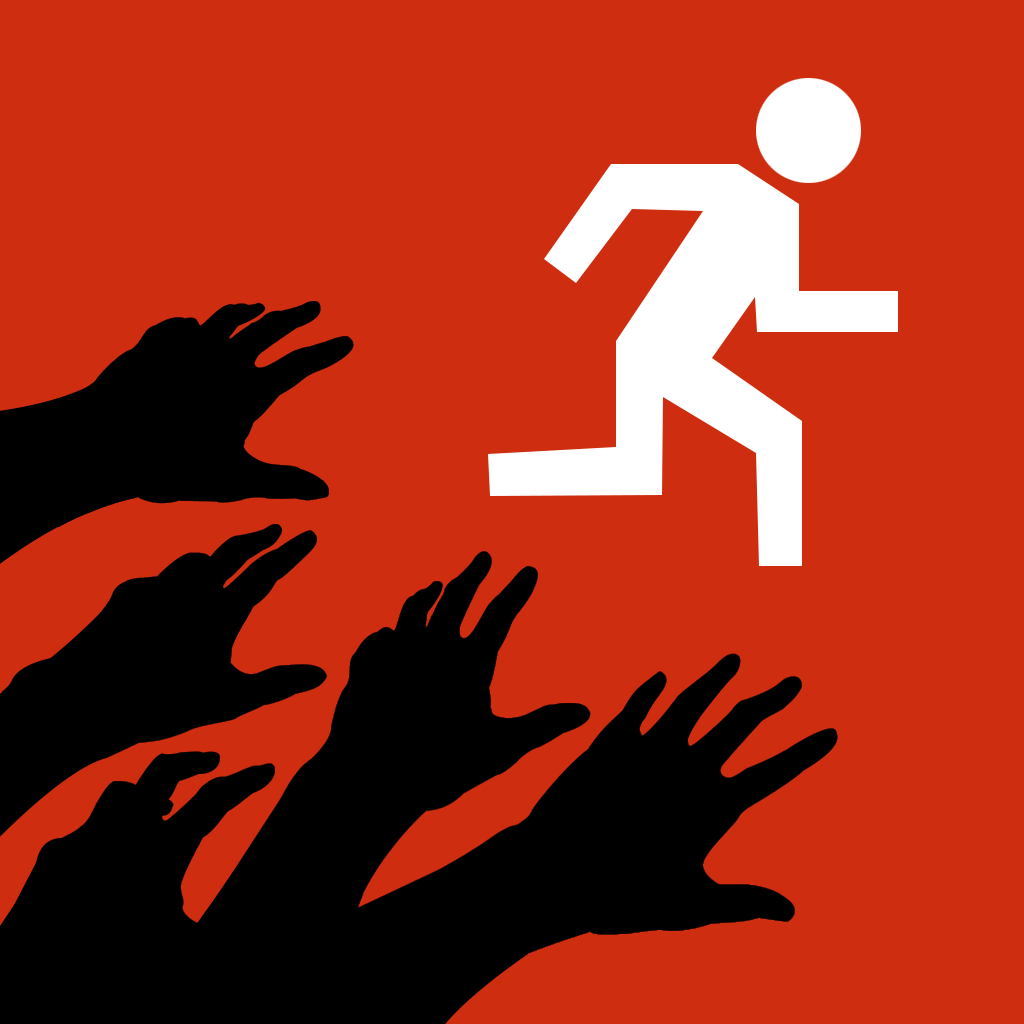
\includegraphics[height=2in]{Figures/zombies-run-logo}
	\caption{The \emph{Zombies, Run!} logo}
\end{figure}

The game narrative places the player in a post-zombie-apocalyptic world, and you are one of few survivors. By going out to run, you'll collect supplies used to build up a base for you and fellow survivors. The game features 200 missions that are narrated mini-stories that drive the plot forward as you build up your base, playing audio clips in between your own music as you run. During your run, it is possible for zombies to appear and chase you, requiring an increased pace. Should you fail to increase your pace and outrun them, they will catch up to you and any supplies you have collected will be lost.

The game uses the device screen minimally to select missions and viewing and sharing your progress between runs, while the game experience is presented through audio. There are no visual augmentations of reality, but the game uses audio clips to perceptibly augment a run. When being chased by zombies, their groans can be heard closing in if you do not run quickly enough, and their distance to you can be felt through the volume and intensity of their sounds. The game also plays a heartbeat in your ears, intended to imitate your own as you run. Southerton \cite{southerton2013zombies} performed an \emph{autoethnography} noting her experiences with the game, and found the heartbeat in particular to add high levels of immersion by adding a sense of urgency, but only during the other audio clips presented by the game.

\begin{figure}[h]
	\centering
	\begin{subfigure}[t]{0.3\textwidth}
		\centering
		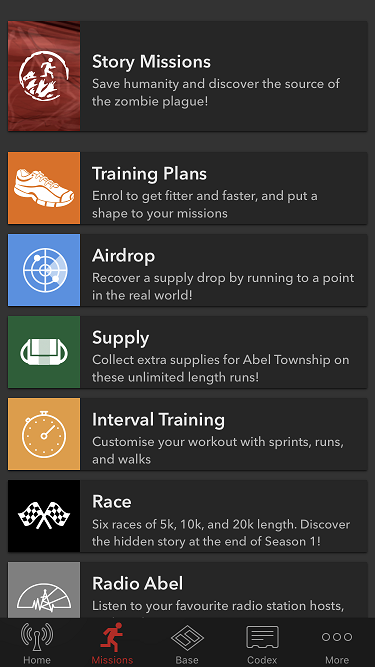
\includegraphics[height=3in]{Figures/zombies-run-activities}
		\caption{Activities available}
	\end{subfigure}
	~
	\begin{subfigure}[t]{0.3\textwidth}
		\centering
		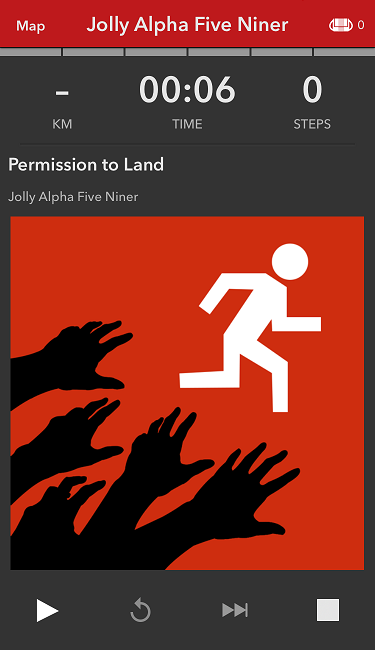
\includegraphics[height=3in]{Figures/zombies-run-mission}
		\caption{The screen while in a mission}
	\end{subfigure}
	~
	\begin{subfigure}[t]{0.3\textwidth}
		\centering
		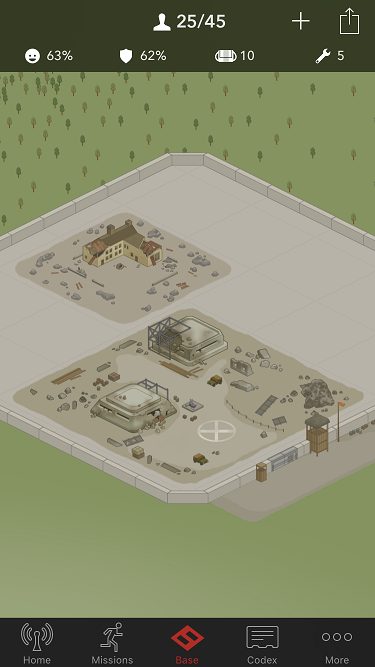
\includegraphics[height=3in]{Figures/zombies-run-base}
		\caption{View of the player's base}
	\end{subfigure}
	\caption{Screenshots of \emph{Zombies, Run!}}
\end{figure}

With basis in Kiefer et al.'s \cite{kiefer2006systematically} paper, Zombies, Run! is a location-based game in that it uses GPS technology to track the player's movements in order to progress in the game by collecting supplies and to escape zombies. It also allows the player to choose a location on a map, and will generate a mission tailored to the distance to that location, called an \emph{Airdrop}. We classify Zombies, Run! as an augmented reality game, with virtual elements (zombies) perceptible in the real world through audio. The game is closest to a chase game, as outrunning the zombies is vital to game progress. The game progresses continually as the player moves, as long as they are on a mission, and a mission can be started at any time. Thus we classify the game as spatially and temporally continuous.

While the game is an exergame in the true sense of being a game with the sole purpose of encouraging physical activity, or more specifically aerobic exercise, the actual impact of the exercise it encourages has been debated. Halushak, an experienced runner, noted in her experience with the game that because of the sparse zombie attacks and high requirement to escape them that the game is more about exercising the players' imagination than to push them to their limits. Halushak's reasoning for this is that the player must increase their pace by at least 20 \% to escape, which is difficult when already running at a quick pace, encouraging an overall lower pace if one wants to be able to escape. Higgins \cite{higgins2016smartphone} in a review of smartphone apps for increasing patients' health and fitness recommended the game for \emph{"healthy patients wanting to start basic aerobic exercise"}, but not any other groups of patients. Other studies (Cowdery et al. \cite{cowdery2015exergame} and Direito et al. \cite{direito2015apps}) performed with the app showed that the physical impact was limited, but that players using these apps were more likely to be motivated to continue their exercise after the control periods. Since these reviews, the game has added more features. Among these features is the ability to adjust the pace increase required to escape zombies, allowing for a more even (and hopefully higher on average) pace, as well game modes such as interval training.

Zombies, Run! was previously a purchasable game, but has since become free to play. It now earns revenue through the sale of premium features (such as increasing the frequency of zombie attacks or additional game modes) and entry into special events.

\section{The Walk}

The Walk is another game from the same developer as \emph{Zombies, Run!}, Six to Start. It is marketed as a \emph{"fitness tracker and game"}, and is sold in the Google Play Store as well as Apple's iOS App Store. It is another story-driven audio-focused augmented reality game, but also features a sort of mini-games on the device screen while you are walking, where you can click objects that momentarily appear which unlock extra bits of the story. The game leads you down a set path in the virtual map of the game, unlocking more of the story as you reach certain points on the map. The game can be played at your own pace and simply continually tracks for how long you have been walking and the number of steps, but awards you badges for performing special actions such as completing an episode with less than 3 hours of breaks between start and finish.

The game's narrative places you in the northern parts of the United Kingdom, where a train station has just been blown up by terrorists. Somehow you mistakenly end up with a package that the terrorists are after, and it becomes your mission to walk across the United Kingdom and deliver it where it belongs. You are guided on your path by a remote secret agent, and have to be wary of dangerous enemy operatives and bystanders suspecting you of being a terrorist.

While the game uses localization technology to progress the virtual game, it is not a location-based game as per Kiefer et al.'s definition, as the virtual map does not reflect the real world, and the GPS technology are only used to measure whether or not you are walking.

\section{Munzee and Stolpejakten}

Munzee (a stylized version of the German word for \emph{coin}) is an scavenger hunt/item hunt game similar to Geocaching, using QR codes and GPS location to register captures as opposed to the physical hidden caches of Geocaching. As in Geocaching, \emph{Munzees} are deployed by players by registering a QR code in the app and placing a waterproof sticker with the code on it in a location of their choosing, which they then register to a map. Munzees are found all over the world, with at least one Munzee present on every continent - including Antarctica \cite{munzee}. Capturing a Munzee awards points to the player who made the capture as well as the player who deployed it.

Stolpejakten (meaning \emph{The Pole Hunt} in Norwegian) is a Norwegian game with a similar concept to Munzee, but instead of stickers attached to poles and other objects, special poles with QR codes attached are placed as markers for the game. The game is marketed as an exergame, with the goal of getting people of all ages and physical conditions active and providing a means of exploration for those who wish to get to know their local community better. They are color coded according to four levels of difficulty, where the \emph{green} poles are the easiest and are reachable by bicycle and wheelchair, and the \emph{black} poles are difficult and require a serious effort in reaching. Capturing a pole gives the user a ticket in a raffle held in the county the pole is located, sponsored by local businesses. Capturing more poles awards more tickets, increasing their odds of winning good prizes such as concert tickets, festival passes or three-course meals at good restaurants.

Both of these games share the two of the same game dimensions as Geocaching, in that they are pure location-based games and are spatially discrete and temporally continuous. They are arguably also item hunt games, Munzee more so than Stolpejakten, as the \emph{Munzees} are much smaller than the poles placed in Stolpejakten. Neither of the games share the puzzle game aspect of Geocaching.

Munzee's revenue comes from the sale of partnerships, as well as the sale of Munzee stickers that players can deploy. Stolpejakten earns their revenue through renting out infrastructure to local organizers and selling memberships to local clubs.

\section{Run an Empire}

Run an Empire is a social exergame where players compete to claim territory for their \emph{empire} through running or jogging. The map is split into \emph{hexes} (hexagonal tiles), and running across a hex stakes a claim to that hex. If your claim is stronger than all other players' claim to the hex, it will be added to your empire. You can strengthen your claim by running across the same hex on another run, and the stronger your claim, the more difficult it will be for intruders to take over your empire. Having more hexes in your empire grant a higher position on the leaderboards. There is both a global leaderboard and a social leaderboard, where the social leaderboard lists the players you are following in the game.

The game focuses on strategy rather than catering only to those of superior physical ability, making the game available and enjoyable for all players. They enable this by limiting each run to one hour, and only allowing one run per 24 hour period. New players are also accommodated by a limit to the strength of a player's claim to a hex, and \emph{tile decay} ensuring that as time passes, a claim weakens if it is not strengthened through active play. The limit also acts as an incentive to expand your area with new routes when your claim to one area is near its limit, an incentive that is further strengthened by the generation of gems randomly on the map when you start a new run. These gems can be used to buy certain items in the game to upgrade your empire. Players also earn coins by running, which encourages play even if the surrounding area is strongly held by an opponent, as coins can be stolen from opponents. These coins, like the gems, can be used to purchase items, and act as secondary points to show a player's achievements over time.

Using Kiefer et al.' game dimensions \cite{kiefer2006systematically}, the game is a mixed reality location-based game, with virtual objects on the map that are not perceivable outside the virtual game environment. It is a strategy game rather than a chase game for the reasons described above, and requires good planning to most efficiently expand your empire. The game area is continuous, and while you can start your first run at any point, the restrictions to length and frequency of runs makes the game temporally discrete. Thus it would seem that Run an Empire is a spatially continuous and temporally discrete game, the class that Kiefer et al. at the time were unable to discover.

Run an Empire is still in a beta state, currently only being available in the United Kingdom and New Zealand, and its main income is from the original Kickstarter campaign that launched the game and other seed money from investors, but their business model includes sale of cosmetic items after the decision to turn the game free to play.

\section{Mobile games}

With hundreds of thousands of games available across iOS \cite{pocketgamerAppstore} and Android, there is a lot of competition for the players' attention. Popular games are often strategy or puzzle games that can be played in short sessions while waiting for something such as the train arriving, or while doing something else such as watching television. Games like Angry Birds and Candy Crush Saga, where you solve small, progressively harder puzzles, have been massively popular in the past and still are. Other social strategy games such as Wordfeud and Game of War are other massively successful games, while action games such as Clash of Clans and Mobile Strike are among the currently top-grossing games on iOS \cite{appAnnieIOS}.

Most of these games are free to play, with revenue coming from in-game advertisements and stores, selling extra lives that allow players to play more levels or items that make certain levels easier to solve.


% Chapter - More about Pokémon and Pokémon GO
\chapter{Pokémon}
\label{chapter:lit-study-pokemon-go}
\lhead{Chapter \ref{chapter:lit-study-pokemon-go}. \emph{Pokémon GO}}

This chapter gives a short introduction to the Pokémon franchise throughout the years, as well as an in-depth description of Pokémon GO and its features.

\section{Pokémon Franchise}

Pokémon is a multi-billion dollar (grossing nearly five trillion Japanese yen) media franchise owned by The Pokémon Company, a Japanese consortium consisting of Nintendo, Game Freak and Creatures. It began in 1996 with a pair of games for the handheld Nintendo gaming console Game Boy, internationally branded as \emph{Pokémon Red} and \emph{Pokémon Blue}. In 1997 an animated television series began airing, which helped popularize the franchise globally. In the twenty years since then, the franchise has released a multitude of games of various genres across all Nintendo gaming consoles, a Trading Card Game, nineteen feature films and several manga series (Japanese comic books). Additionally, Pokémon merchandise of all sorts is sold almost everywhere, ranging from plush toys to office equipment with Pokémon art, and the brand is licensed for all sorts of content.

The concept of Pokémon revolves around the namesake monsters which exist alongside humans in the fictional universe that is the setting of the franchise. In the Pokémon universe, all life forms besides humans are Pokémon, taking familiar forms such as dogs, rodents, insects, birds and fish, as well as traditionally less-than-sentient objects such as plants, magnets or piles of muck. The Pokémon have supernatural powers, such as generating electricity, controlling the weather or breathing fire, which they use to attack and defend themselves. Humans catch and tame these Pokémon and use them as pets, companions and assistants, but the main focus of both the games and other media are the \emph{Pokémon trainers}, who use Pokémon to battle other Pokémon trainers.

The slogan of the franchise is \emph{"Gotta catch 'em all"}, referring to the desire of the main protagonist of the series to become the world's best Pokémon trainer by capturing all the different species of Pokémon available, on his journey to become the champion of the Pokémon League. The two concepts of catching \emph{"'em all"} and battling other trainers are present in almost all of the games, and throughout the \emph{anime} (the animated television series), movies and manga.

\section{Pokémon GO In-Depth}
\label{sec:pokemon-go-in-depth}

Pokémon GO is an augmented reality location-based game. It places the monsters of the franchise out into the real world, making them visible and catchable through Android and iOS smart phones. The game also features Pokémon battling in special locations known as \emph{gyms}. The game shows a map of the surrounding area with the player's avatar placed onto it in the player's current physical location, determined using GPS localization. To move around in the game, the player has to physically move in the real world.

Various Pokémon will appear on the map around the player at certain times, and remain there for up to 30 minutes or until the player attempts to catch it and either succeeds or fails enough times for the Pokémon to flee. Pokémon that spawn naturally are visible for all players, and one player catching it does not affect its availability for other players, but players can only see Pokémon within a radius of roughly 30 meters.

To catch Pokémon, the player, or \emph{trainer} as players are called, throws so-called Pokéballs at the Pokémon. A visual indicator, represented by a colored circle, shows at what time the throw has the greatest chance of successfully catching the Pokémon. Pokéballs exist in three different varieties found at \emph{Pokéstops}, which we will cover shortly. Using a better ball will increase the odds of capturing the Pokémon, but they are also less commonly dropped by Pokéstops. \emph{Razzberries}, another item gained at Pokéstops, are single-use items that increase the capture rate of the next Pokéball that hits the Pokémon.

In the capture view, the player can toggle \emph{AR mode} on or off, switching between a view where the Pokémon is superimposed on the view of the device camera, or a standard background of an animated forest. The capture view also features a camera function that hides the UI and allows the player to take fun or interesting photos of the Pokémon, typically used in conjunction with AR mode, putting players in a situation resembling that of the Nintendo 64 game \emph{Pokémon Snap}, where players were tasked to take interesting photos of Pokémon.

\begin{figure}[h]
	\centering
	\begin{subfigure}[t]{0.3\textwidth}
		\centering
		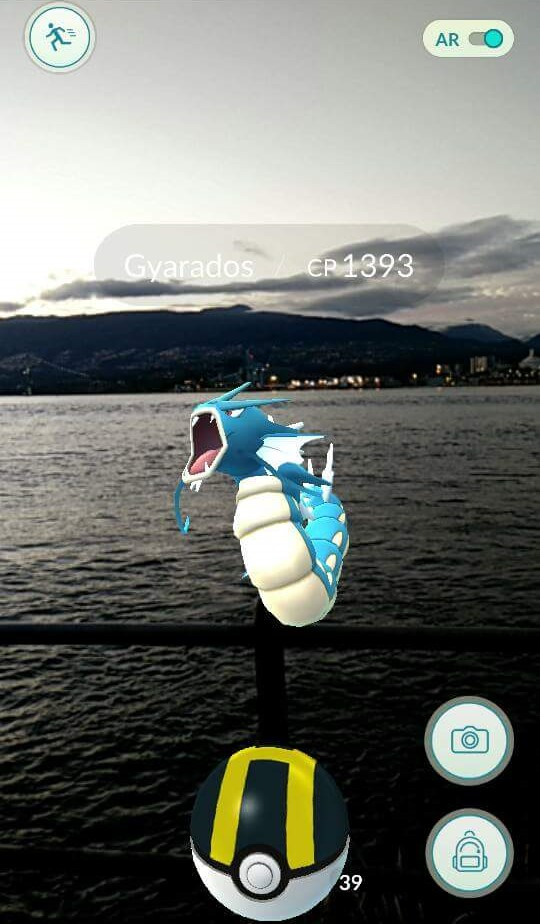
\includegraphics[height=3in]{Figures/pogo-gyarados-chocolatechoux}
		\caption{A wild \emph{Gyarados} in its natural habitat, by Reddit user chocolatechoux}
	\end{subfigure}
	~
	\begin{subfigure}[t]{0.3\textwidth}
		\centering
		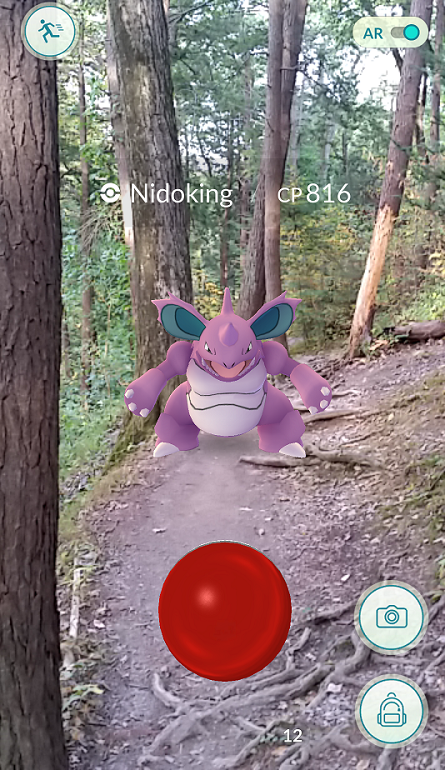
\includegraphics[height=3in]{Figures/pogo-nidoking-blocking-trail-GCBill}
		\caption{A wild \emph{Nidoking} in its natural habitat, by Reddit user GCBill}
	\end{subfigure}
	~
	\begin{subfigure}[t]{0.3\textwidth}
		\centering
		
\includegraphics[height=3in]{Figures/pogo-catch-gotcha}
		\caption{A successful catch}
	\end{subfigure}
	\caption{Capturing a Pokémon}
\end{figure}

Pokéstops are special locations, and are a subset of Ingress' portals, described in Section \ref{sec:ingress}. The main feature of these Pokéstops is to dispense consumable items such as all varieties of the aforementioned Pokéballs (Pokéballs, Great Balls and Ultra Balls), as well as Razzberries, all types of \emph{Potions} (regular, Super, Hyper and Max) and both types of \emph{Revives} (regular and Max), with higher level items being less frequent drops. Pokéstops can also drop Pokémon eggs. Potions and Revives of all kinds are used to heal Pokémon that have been damaged in battle. The player can claim items from each Pokéstop once every five minutes, and does so by pressing the Pokéstop and spinning the \emph{photo disc}.

\begin{figure}[h]
	\centering
	\begin{subfigure}[t]{0.45\textwidth}
		\centering
		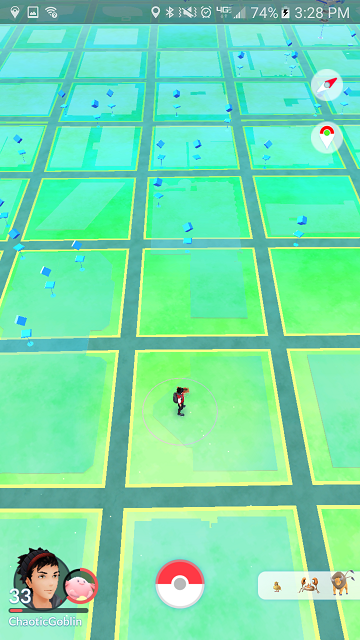
\includegraphics[height=3in]{Figures/pogo-map-of-ingress-equivalent}
		\caption{Pokémon GO, by Reddit user chaoticgoblin}
	\end{subfigure}
	~
	\begin{subfigure}[t]{0.45\textwidth}
		\centering
		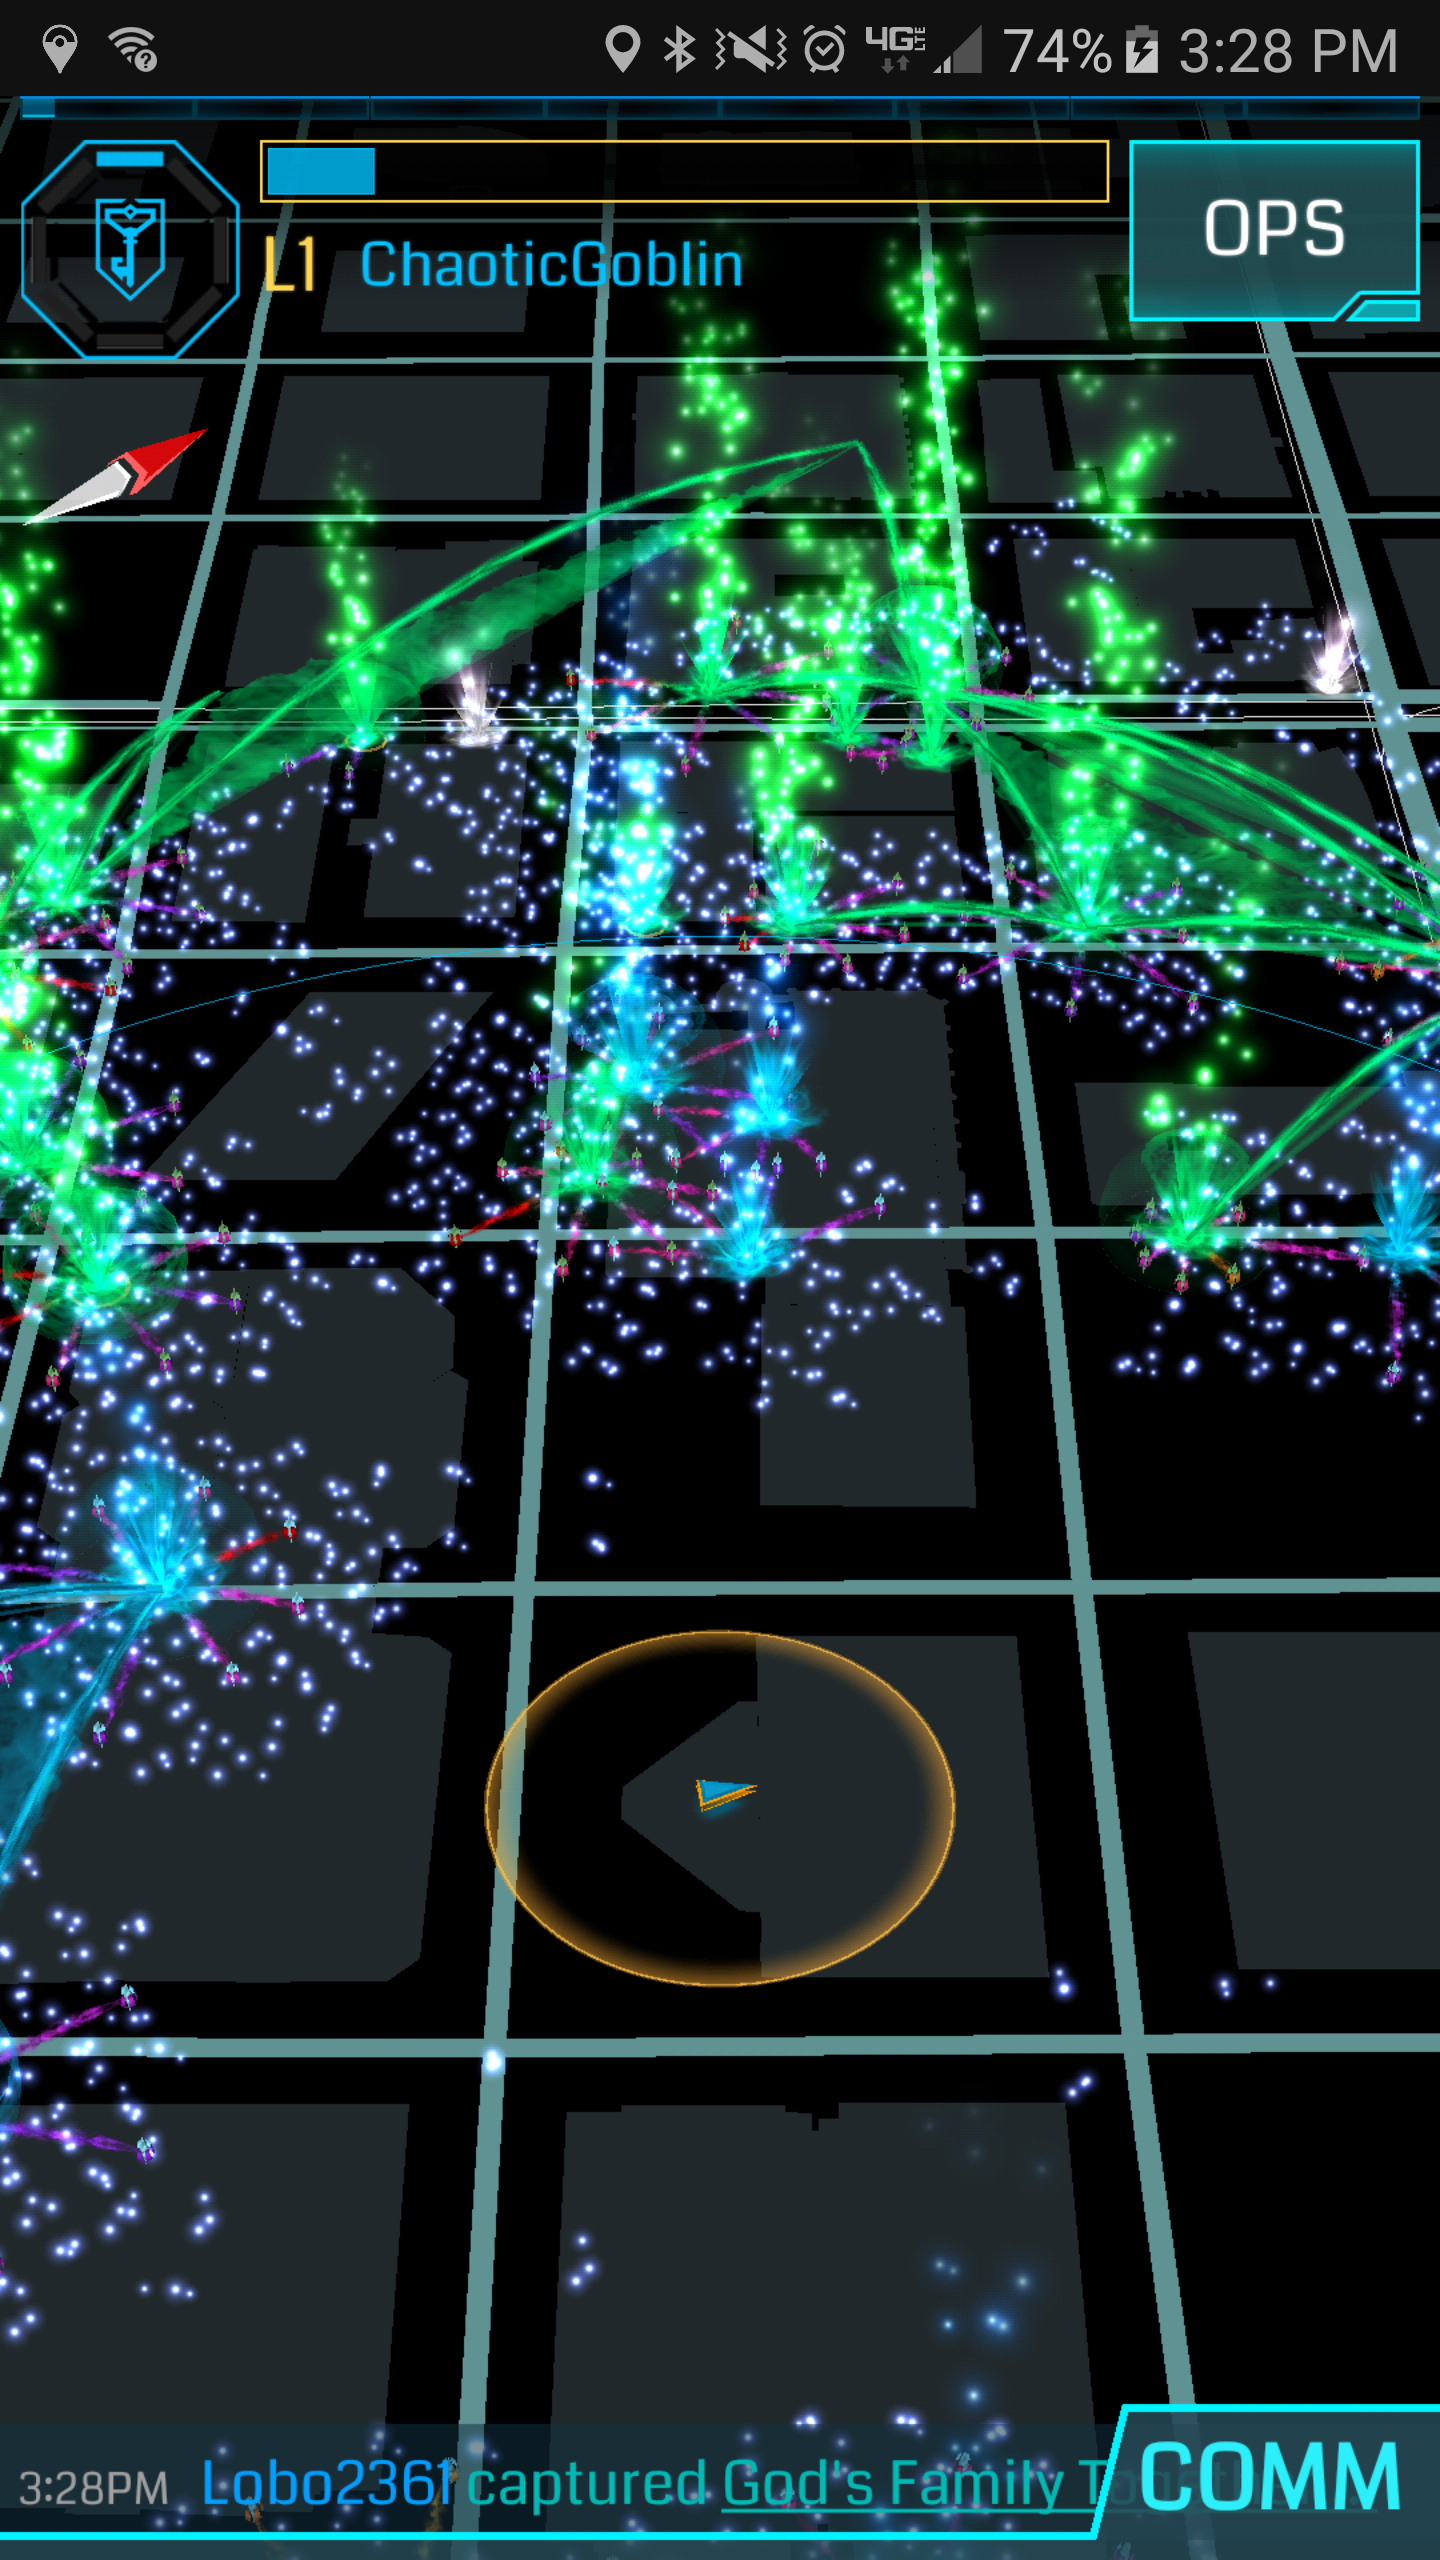
\includegraphics[height=3in]{Figures/chaoticgoblin-ingress-screenshot}
		\caption{Ingress, by Reddit user chaoticgoblin}
	\end{subfigure}
	\caption{The same location in Pokémon GO and Ingress}
\end{figure}

A secondary feature of Pokéstops is that players can place \emph{Lure Modules} on them, an item purchasable in the store that lures one semi-random Pokémon to the stop for two minutes every five minutes, over a span of 30 minutes. These Pokémon are visible to all nearby trainers, and can be any Pokémon of the species that are eligible to spawn in the area. Pokéstops are also featured in the player's \emph{tracker}, a feature that allows players to see what Pokémon are currently in the area. It is split into two parts, \emph{Nearby} and \emph{Sightings}. Pokémon in the \emph{Nearby} category are listed together with the Pokéstop closest to their location, while Pokémon in the \emph{Sightings} category are in your immediate vicinity and not within range of a Pokéstop.

\begin{figure}[h]
	\centering
	\begin{subfigure}[t]{0.45\textwidth}
		\centering
		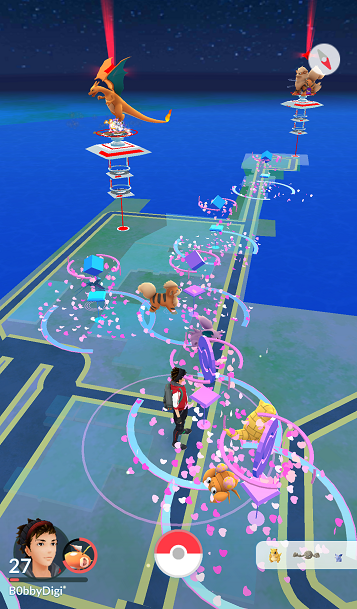
\includegraphics[height=3in]{Figures/pogo-santa-monica-lures-bobby1211}
		\caption{Lured Pokéstops at Santa Monica Pier, by Reddit user Bobby1211}
	\end{subfigure}
	~
	\begin{subfigure}[t]{0.45\textwidth}
		\centering
		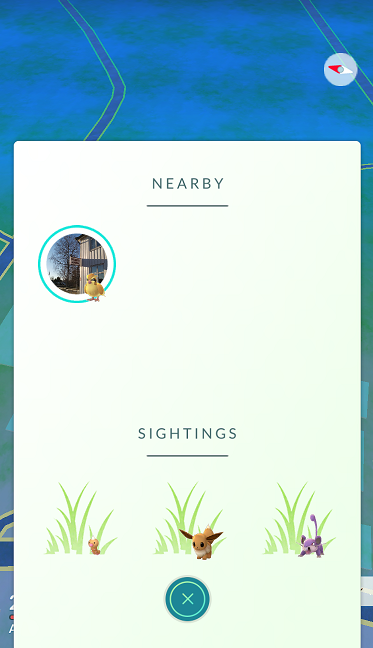
\includegraphics[height=3in]{Figures/pogo-tracker}
		\caption{The in-game Pokémon tracker}
	\end{subfigure}
	\caption{Secondary features of Pokéstops}
\end{figure}

Basic Pokéballs can also be purchased in the in-game shop, using \emph{coins}. These coins can be purchased in the same shop using real money, or earned through gym battling, which we will cover in the next paragraph. The shop also sells \emph{Incense}, \emph{Lucky Eggs}, lure modules and \emph{Egg Incubators}, as well as upgrades to Pokémon or item storage.

Incense resemble lure modules in that they attract semi-random Pokémon, but are deployed on the player rather than a Pokéstop. The incense lasts for 30 minutes, and remains on the player as they move around, but any Pokémon it spawns are visible only to the player who used the incense. These Pokémon are shown with a purple cloud circling around them on the map. Incense will spawn Pokémon at a rate depending on the player's activity: a Pokémon will spawn every fives minutes while the player is standing still, or every minute while the player is moving, if they have moved at least 200 meters since the last check.

Lucky eggs double the amount of experience points gained by the player for the next 30 minutes. Experience points can be gained by catching a Pokémon, hatching an egg, evolving a Pokémon or battling in a gym. Additional experience is awarded for adding a new \emph{Pokédex entry}, making a particularly good throw at an opportune time while catching a Pokémon, defeating an entire gym, or if you are making your first catch of the day, as well as for every 100 Pokémon you catch of a species. Earning a new Pokédex entry is done by capturing, hatching or evolving a Pokémon you did not previously have, playing into the \emph{"gotta catch 'em all"} slogan.

Egg incubators are used to incubate Pokémon eggs. Incubating an egg allows it to be hatched, and each egg requires either 2, 5 or 10 kilometers of walking while incubated to hatch. Each type of egg, with types determined by the distance required to hatch it, can hatch into a different set of Pokémon, with 10 km eggs containing some of the rarest and strongest Pokémon in the game, such as \emph{Snorlax} and \emph{Lapras}. In addition to a new Pokémon and some experience points, hatching an egg awards an amount of \emph{Stardust} and \emph{Candy} proportional to the effort required to hatch the egg.

\begin{figure}[h]
	\centering
	\begin{subfigure}[t]{0.3\textwidth}
		\centering
		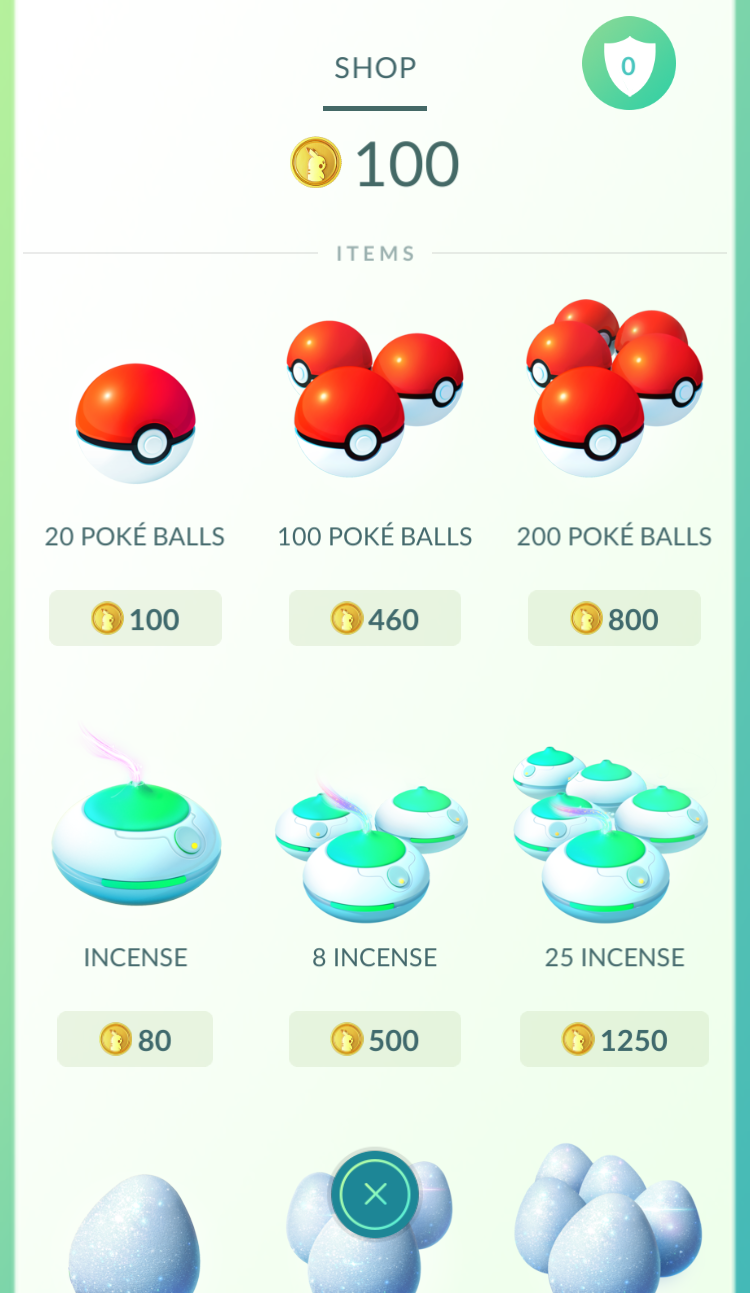
\includegraphics[height=3in]{Figures/pogo-shop}
		\caption{A view of the in-game store}
	\end{subfigure}
	~
	\begin{subfigure}[t]{0.3\textwidth}
		\centering
		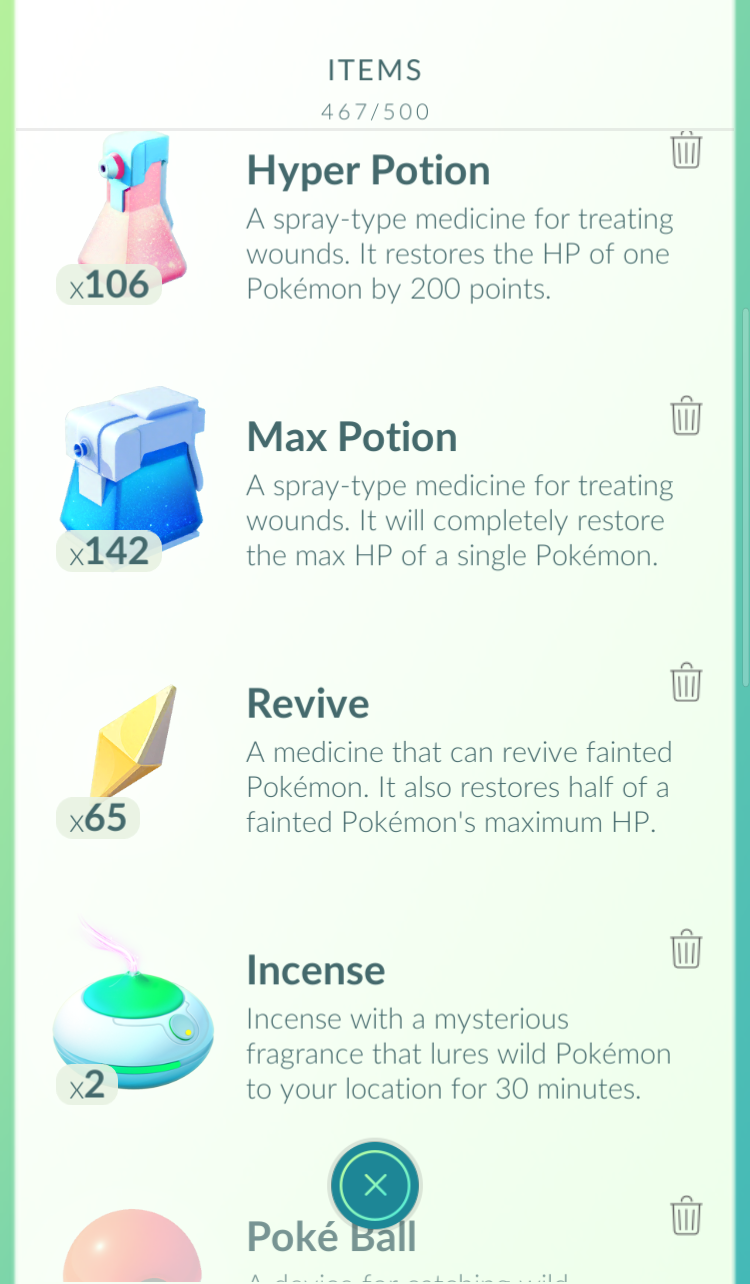
\includegraphics[height=3in]{Figures/pogo-inventory}
		\caption{A view of the player inventory}
	\end{subfigure}
	~
	\begin{subfigure}[t]{0.3\textwidth}
		\centering
		
\includegraphics[height=3in]{Figures/pogo-incubated-eggs}
		\caption{The currently carried eggs with some incubated}
	\end{subfigure}
	\caption{Items and eggs}
\end{figure}

Stardust, which is also gained by catching Pokémon, is used to \emph{Power up} Pokémon. The amount of stardust required to power up a Pokémon increases the stronger the Pokémon gets, ranging from 200 stardust at its weakest to 10 000 near its strongest. Catching a Pokémon always yields 1000 stardust, and the extent to which a Pokémon can be powered up depends on the player's level. Powering up a Pokémon increases its combat potential by making it deal more damage (increased \emph{Combat Power (CP)}) and able to take more damage (\emph{increased health/hit points (HP)}).

Candy is the second resource related to the Pokémon themselves. Each evolution line of Pokémon has their own type of candy, named after the base form of the species - for example, Pidgey candy is used for Pidgey as well as its evolutions Pidgeotto and Pidgeot. Candy is earned through capturing a Pokémon (yielding three candy of the appropriate type), hatching a Pokémon (yielding from 5 to 32 candy depending on the type of the egg), \emph{transferring} or evolving a Pokémon (each yielding one candy). Transferring a Pokémon donates it to Professor Willow, the Pokémon expert guiding you through the game, and is the game's way of making the act of deleting a Pokémon immersive. Candy is used alongside stardust to power up a Pokémon, the required amount ranging from 1 to 15 depending on the current power level of the Pokémon. It is also used to evolve a Pokémon to a new species at a later stage in the evolution chain. Evolution is not a new concept for Pokémon GO, and evolution chains has been a part of the franchise since the beginning, with most Pokémon having between one and three stages. A single Pokémon (at a time) can be chosen as the player's \emph{buddy}, earning the player an additional candy every few kilometers they walk, the exact distance required varying from one to five kilometers depending on the species of the buddy.

\begin{figure}[h]
	\centering
	\begin{subfigure}[t]{0.3\textwidth}
		\centering
		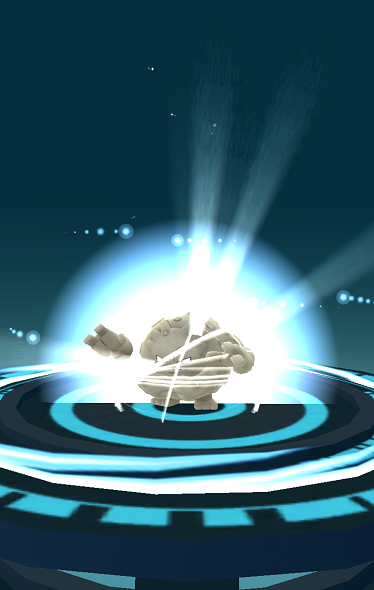
\includegraphics[height=2.8in]{Figures/pogo-evolving-graveler}
		\caption{Evolving a \emph{Graveler}}
	\end{subfigure}
	~
	\begin{subfigure}[t]{0.3\textwidth}
		\centering
		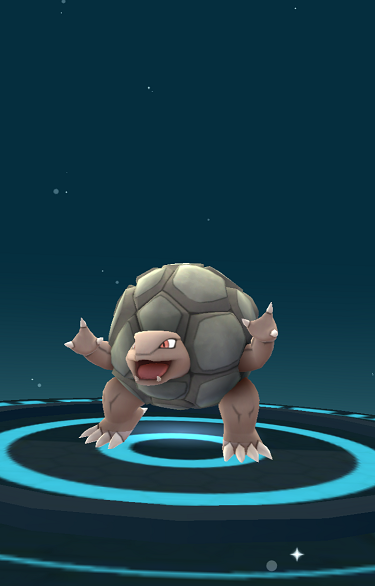
\includegraphics[height=2.8in]{Figures/pogo-evolved-golem}
		\caption{Evolved into a \emph{Golem}}
	\end{subfigure}
	~
	\begin{subfigure}[t]{0.3\textwidth}
		\centering
		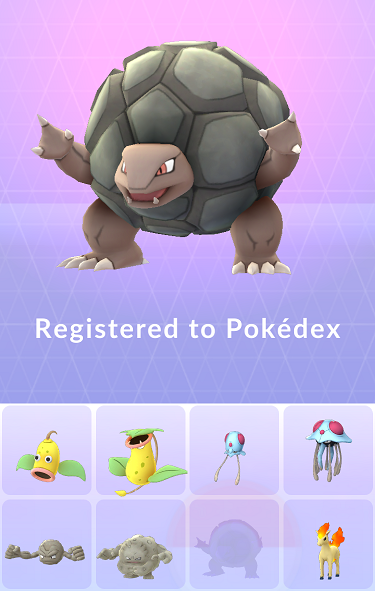
\includegraphics[height=2.8in]{Figures/pogo-new-poke}
		\caption{New Pokédex entry}
	\end{subfigure}
	\caption{Evolving a Pokémon}
\end{figure}

When a player reaches level 5, they can approach a gym and choose to join one of the three teams in the game: \emph{Valor} (the red team), \emph{Mystic} (the blue team) or \emph{Instinct} (the yellow team). The player can then claim gyms for their own team by placing one of their Pokémon in an empty gym to defend it against attackers from other teams. A gym can be leveled up to a max of level 10, and each gym level opens up an additional spot for a Pokémon from the controlling team, with a limit of one Pokémon per player at each gym. Leveling up a gym is done by \emph{training} it through friendly battle. To take down an enemy gym, players can battle it with their own Pokémon, choosing a team of up to six of their Pokémon.

A Pokémon battle is a last-Pokémon-standing fight, where attackers fight one defender at a time. When attacking an opposing gym, multiple players from any of the teams not currently controlling the gym can fight together to take down the defenders, while training a friendly gym limits the battle to a one-on-one fight. Pokémon have two \emph{attacks} or \emph{moves}, each randomly selected from a pool of eligible moves upon acquiring the specific Pokémon. The Pokémon use a \emph{typing} system where each Pokémon has one or two "elemental" types, and each move having one type. There are 18 different types, using a rock-paper-scissors scheme where some types are strong against certain types and weak against others, and neutral against the rest. As an example, fire moves are strong against grass Pokémon, neutral against flying Pokémon and weak against water Pokémon. Strong moves deal 25 \% increased damage, while weak moves deal 25 \% reduced damage. Having double \emph{type advantage}, such as a water move against a Pokémon with both rock and ground types, leads to an even stronger attack. The strength can be further increased by using a move with the same type as the Pokémon using it, such as a water Pokémon using a water move. Figure \ref{fig:pokemon-stats} shows the fact sheet for a single captured Pokémon, a \emph{Slowpoke} with a psychic attack (\emph{Confusion}) and a water attack (\emph{Water Pulse}).

\begin{figure}[h]
	\centering
	\begin{subfigure}[t]{0.3\textwidth}
		\centering
		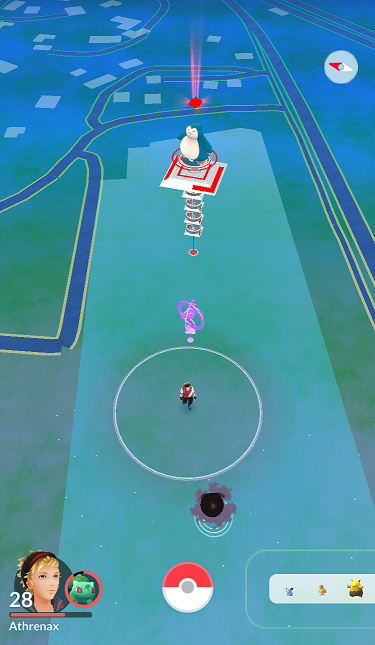
\includegraphics[height=3in]{Figures/pogo-near-gym}
		\caption{A gym as seen on the map, with the strongest Pokémon in the gym displayed on top}
	\end{subfigure}
	~
	\begin{subfigure}[t]{0.3\textwidth}
		\centering
		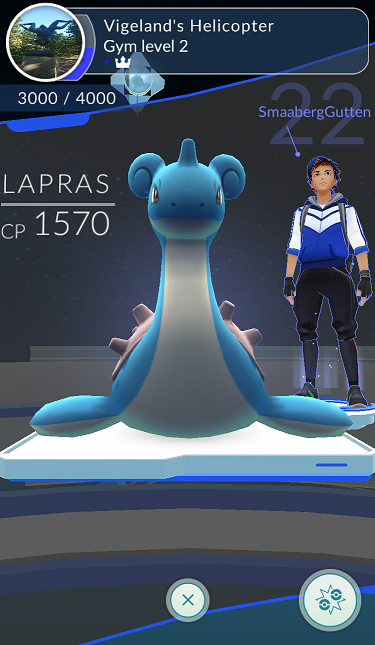
\includegraphics[height=3in]{Figures/pogo-trainer-in-gym}
		\caption{The lobby of a gym, showing one of its trainers with the Pokémon stationed there}
	\end{subfigure}
	~
	\begin{subfigure}[t]{0.3\textwidth}
		\centering
		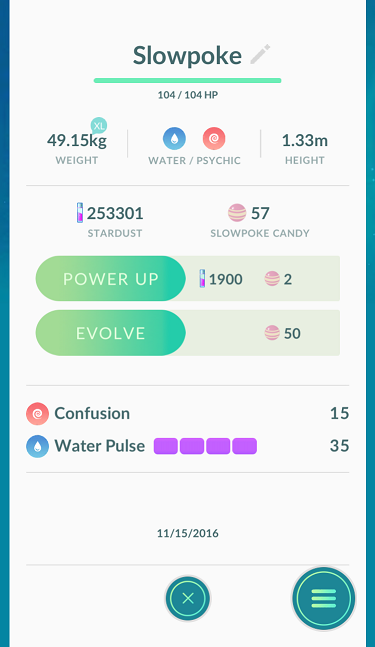
\includegraphics[height=3in]{Figures/pogo-moves-and-resources}
		\caption{A single captured Pokémon's fact sheet}
		\label{fig:pokemon-stats}
	\end{subfigure}
	\caption{Gyms and Pokémon}
\end{figure}

Most actions in the game earn progress towards a badge, shown in Figure \ref{fig:pogo-badges}. Some of these badges increase the odds of catching specific types of Pokémon based on the level of the badge.

\begin{figure}[h]
	\centering
	\begin{subfigure}[t]{0.3\textwidth}
		\centering
		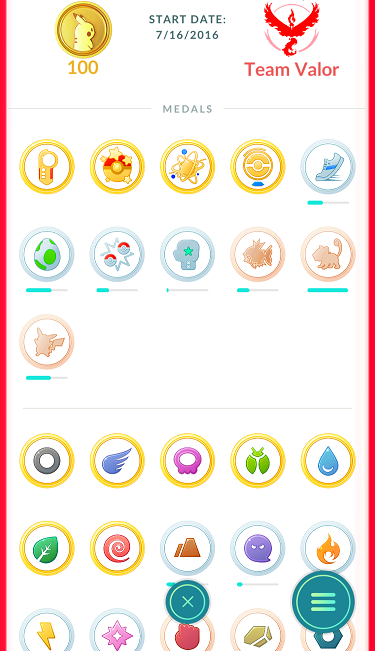
\includegraphics[height=3in]{Figures/pogo-badges}
		\caption{An overview of the various badges collected}
	\end{subfigure}
	~
	\begin{subfigure}[t]{0.3\textwidth}
		\centering
		
\includegraphics[height=3in]{Figures/pogo-jogger-badge}
		\caption{The \emph{Jogger} badge, showing current progress}
	\end{subfigure}
	~
	\begin{subfigure}[t]{0.3\textwidth}
		\centering
		
\includegraphics[height=3in]{Figures/pogo-collector-badge}
		\caption{The \emph{Collector} badge, showing current progress}
		\label{fig:pogo-badges}
	\end{subfigure}
	\caption{Badges}
\end{figure}

Using Kiefer et al.'s \cite{kiefer2006systematically} game dimensions, Pokémon GO is an augmented reality location-based game, with Pokémon being perceivable in the real world through the AR mode in the application. It can be played anywhere and at any time, making it spatially and temporally continuous. Even if there are no Pokéstops or spawns nearby, the player can still earn distance for their incubated eggs and their buddy. The game is arguably primarily an item hunt game, with the capture of Pokémon being the main goal, although the area which the user has to search is scaled up to be the area within range of the tracker rather than an area defined by coordinates where the player has to search in bushes, under benches or similar in the very specific area. However, the game is also a strategy game, with multiple areas of the game requiring some form of strategy to play efficiently. Battles require a good portion of planning to win reliably and effectively, and resource management is important to not run out of consumables. Resource management is also important with stardust and candy, as a player will gain much less of these resources than what is needed should they wish to power up and evolve everything. To evolve a single Pidgey, a player will have to catch at least two others, and stronger evolutions cost even more candy.
